
\subsection{Lustro i~rewers. Węzły skrętne i zwierciadlane}
\begin{definition}[lustro]
% DICTIONARY;mirror;lustro/lustrzany;węzeł
\index{lustro}%
\index{węzeł!lustrzany}% TODO: to się może mylić ze zwieciadlanym
    Niech $L$ będzie zorientowanym splotem.
    Splot $mL$ powstały przez odbicie splotu $L$ względem dowolnej płaszczyzny nazywamy lustrem.
\end{definition}

Niektórzy mówią o splotach lustrzanych albo odbiciach lustrzanych.

\begin{definition}[rewers]
% DICTIONARY;reverse;rewers/odwrotny;węzeł
\index{rewers}%
\index{węzeł!odwrotny}%
    Niech $L$ będzie zorientowanym splotem.
    Splot $rL$ powstały przez odwrócenie orientacji wszystkich ogniw splotu $L$ nazywamy rewersem.
\end{definition}

Podobnie, tu mówi się o splotach odwrotnych albo odwrotnościach.

\begin{comment}
\begin{figure}[H]
    \begin{minipage}[b]{.32\linewidth}
        \centering
        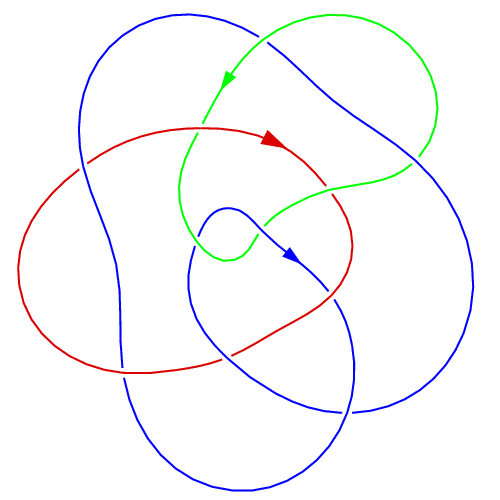
\includegraphics[width=\linewidth]{../data/link_mirror.png}
        \subcaption{lustro $mL$}
    \end{minipage}
    \begin{minipage}[b]{.32\linewidth}
        \centering
        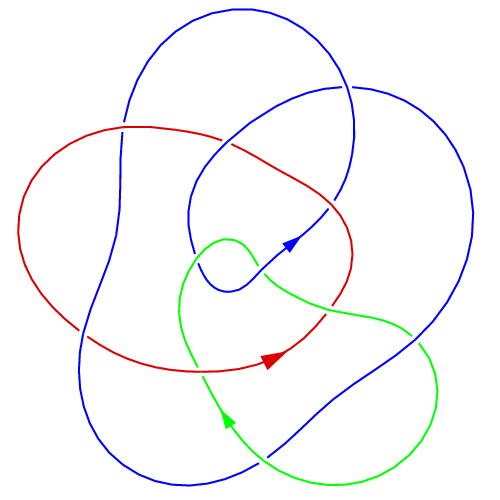
\includegraphics[width=\linewidth]{../data/link.png}
        \subcaption{przykładowy splot $L$}
    \end{minipage}
    \begin{minipage}[b]{.32\linewidth}
        \centering
        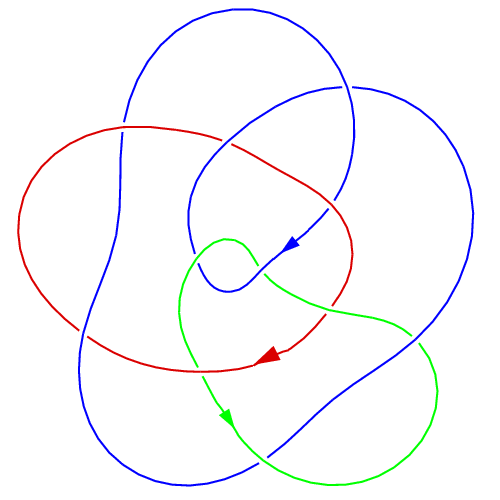
\includegraphics[width=\linewidth]{../data/link_reverse.png}
        \subcaption{rewers $rL$}
    \end{minipage}
\end{figure}
\end{comment}

Na lewym obrazku odbiliśmy diagram względem poziomej prostej, innym sposobem na otrzymanie lustra jest odwrócenie wszystkich skrzyżowań, co odpowiada odbijaniu względem płaszczyzny papieru.
Zauważmy, że wykonując powyższe operacje na węźle możemy otrzymać mniej niż czterech różne obiekty ($L$, $mL$, $rL$, $mrL$) -- na przykład trójlistnik jest własnym rewersem, ale nie lustrem.

Wyróżniamy pięć typów symetrii węzłów:

% DICTIONARY;chiral;skrętny/chiralny;węzeł
\begin{definition}[całkowicie chiralny albo skrętny]
\index{węzeł!chiralny}%
\index{węzeł!skrętny|see {węzeł lustrzany}}%
    Węzły $K$, $rK$, $mK$ są parami nierównoważne. % chiral 9_32
\end{definition}

% DICTIONARY;reversible;odwracalny;węzeł
\begin{definition}[odwracalny]
    \index{węzeł!odwracalny}%
    Węzły $K \cong rK$ są równoważne. % reversible 3_1
\end{definition}

% DICTIONARY;achiral/amphicheiral;zwierciadlany;węzeł
\begin{definition}[ujemnie zwierciadlany]
    \index{węzeł!zwierciadlany}%
    Węzły $K \cong mrK$ są równoważne. % negative amphicheiral 8_17
\end{definition}

\begin{definition}[dodatnio zwierciadlany]
    Węzły $K \cong mK$ są równoważne. % positive amphicheiral 12a_427
\end{definition}

\begin{definition}[całkowicie zwierciadlany]
    Węzły $K, rK, mK$ są parami równoważne. % fully amphicheiral 4_1
\end{definition}

\begin{example}
    Węzeł $9_{32}$ jest całkowicie skrętny.
\end{example}

% Całkowicie skrętne są też między innymi wszystkie węzły torusowe.
% TODO: wiki pisze Each nontrivial torus knot is prime[4] and chiral.[2]

\begin{example}
    \label{exm:trefoil_is_chiral}
    Trójlistnik jest odwracalny, ale nie zwierciadlany.
\end{example}

Po raz pierwszy odkrył to Max Dehn \cite{dehn14} w 1914 roku.
Oto, jak tego dokonał.
% równik = equator
% równoleżnik = parallel (of latitude), najdłuższy równoleżnik to równik
% południk = meridian (of longitude)
% https://math.stackexchange.com/questions/2511364/how-did-dehn-prove-that-the-trefoil-is-chiral myli te pojęcia: pisze o meridian i longitude, kiedy oryginalna praca Dehna operowała na longitude i latitude
Iloraz grafu Cayleya dla grupy podstawowej trójlistnika, $G = \pi_1(S^3 - K)$, zanurza się w~produkt $\mathbb H^2 \times \R$, co pozwala wyznaczyć grupę zewnętrznych automorfizmów grupy $G$, $\Z/2\Z$.
\index{grupa!podstawowa}
% DICTIONARY;latitude;szerokość geograficzna;geografia
% DICTIONARY;longitude;długość geograficzna;geografia
% DICTIONARY;meridian (of longitude);południk;geografia
% DICTIONARY;parallel (of latitude);równoleżnik;geografia
% DICTIONARY;---;geografia;-
Korzystając z~południków i~równoleżników pokazał następnie, że nietrywialny automorfizm zewnętrzny odwraca orientację przestrzeni otaczającej.

My przekonamy się o~tym po wyznaczeniu wielomianu Jonesa trójlistnika, patrz wniosek \ref{cor:joines_of_amphicheiral}.

\begin{example}
    Węzeł $8_{17}$ jest zwierciadlany ujemnie, ale nie odwracalny.
\end{example}

Sześćdziesiąt lat temu matematycy nie byli pewni, czy węzły nieodwracalne w~ogóle istnieją \cite[problem 10]{fox62};
obecnie wiadomo, że nieodwracalne są prawie wszystkie węzły (Murasugi \cite[s.~46]{murasugi96}).
\index[persons]{Murasugi, Kunio}%
W~roku 1962 Ralph Fox wskazał kilku kandydatów do tego tytułu.
\index[persons]{Fox, Ralph}%
Hale Trotter odkrył rok później nieskończoną rodzinę nieodwracalnych precli, patrz \ref{prp:pretzel_not_invertible}.
\index[persons]{Trotter, Hale}%

% MAKOTO SAKUMA - A SURVEY OF THE IMPACT OF THURSTON’S WORK ON KNOT THEORY
% Hartley [129] realized that one can apply this method to the problem of identifying noninvertible knots, as follows. Suppose no automorphism of Γ maps γ to γ−1. Then the set R(G(K), Γ, γ) is possibly different from the set R(G(K), Γ, γ−1), and there is a chance to show noninvertibility of K by comparing the homology invariants associated with φ ∈ R(G(K), Γ, γ) with those associated with φ′ ∈ R(G(K), Γ, γ−1). Hartley showed that this method is quite effective: he completely determined the 36 non-invertible knots up to 10 crossings claimed by Conway to be noninvertible.

\begin{example}
    Węzeł $12a_{427}$ jest zwierciadlany dodatnio, ale nie odwracalny.
\end{example}

Żaden inny węzeł pierwszy o mniej niż 13 skrzyżowaniach nie ma tej cechy.

\begin{example}
\label{property_of_eight_knot}%
    Ósemka $4_1$ jest całkowicie zwierciadlana.
\end{example}

To najprostszy typ symetrii, wystarczy jawnie wskazać przekształcenie między diagramem węzła, jego lustra oraz odwrotności.

Tait odnosił wrażenie, że zwierciadlane węzły mają parzysty indeks skrzyżowań, ale Hoste, Thistlethwaite znaleźli w~1998 kontrprzykład o~piętnastu skrzyżowaniach, $15_{700}$. % wg https://mathworld.wolfram.com/AmphichiralKnot.html
(Czwarta) hipoteza Taita jest prawdziwa dla węzłów pierwszych, alternujących.

\begin{proposition}[10.4.4 w \cite{kawauchi96}, \ref{cor:joines_of_amphicheiral} u nas]
    Niech $K$ będzie węzłem zwierciadlanym.
    Wtedy
    \begin{align}
        V(t) & = V(1/t) \\
        P(a, z) & = P(1/a, z) \\
        F(a, z) & = F(1/a, z),
    \end{align}
    gdzie $\jones, P, F$ oznacza kolejno wielomian Jonesa, HOMFLY oraz Kauffmana.
    Równość $\conway(z) = \conway(-z)$ zachodzi dla wszystkich węzłów, zwierciadlanych lub nie.
\end{proposition}

Poniższa tabela oparta jest (kolejno) o~ciągi
\href{https://oeis.org/A051766}{51766},
\href{https://oeis.org/A051769}{51769},
\href{https://oeis.org/A051768}{51768},
\href{https://oeis.org/A051767}{51767},
\href{https://oeis.org/A052400}{52400},
z bazy danych ``The On-Line Encyclopedia of Integer Sequences'' (OEIS).

\begin{table}[h]
    \centering
    \begin{tabular}{@{}*{20}l@{}} \toprule
        skrzyżowania & 3 & 4 & 5 & 6 & 7 & 8 & 9 & 10 & 11 & 12 & 13 & 14 \\ \midrule
        całkowicie skrętne & 0 & 0 & 0 & 0 & 0 & 0 & 2 & 27 & 187 & 1103 & 6919 & 37885 \\
        odwracalne & 1 & 0 & 2 & 2 & 7 & 16 & 47 & 125 & 365 & 1015 & 3069 & 8813 \\
        $-$ zwierciadlane & 0 & 0 & 0 & 0 & 0 & 1 & 0 & 6 & 0 & 40 & 0 & 227 \\
        $+$ zwierciadlane & 0 & 0 & 0 & 0 & 0 & 0 & 0 & 0 & 0 & 1 & 0 & 6 \\
        zwierciadlane & 0 & 1 & 0 & 1 & 0 & 4 & 0 & 7 & 0 & 17 & 0 & 41 \\
        \bottomrule
        \hline
    \end{tabular}
    \caption{Liczba węzłów o~poszczególnych typach symetrii}
\end{table}

\begin{definition}[10.3.2 w \cite{kawauchi96}]
    Niech $K \subseteq S^3$ będzie węzłem.
    Jeśli istnieje inwolucja pary $(S^3, K)$, która zachowuje orientację sfery, ale odwraca orientację węzła, to węzeł $K$ nazywamy silnie odwracalnym.
\end{definition}

\begin{proposition}
    Jeśli węzeł jest silnie odwracalny, to jest też odwracalny.
\end{proposition}

\begin{proof}
    Oczywiste!
\end{proof}

Hipotezę, że implikacja odwrotna jednak zachodzi, postawił Montesinos \cite[problem 1.6]{kirby78}, on też zdefiniował klasę silnie odwracalnych węzłów \cite{montesinos75}.
\index[persons]{Montesinos, José}%
Jednakże...

\begin{proposition}
    Istnieją odwracalne węzły, które nie są silnie odwracalne.
\end{proposition}

\begin{proof}
\index[persons]{Hartley, Richard}%
\index[persons]{Whitten, Wilbur}%
    Stosowne przykłady podali niezależnie od siebie Hartley \cite{hartley80} oraz Whitten \cite{whitten81}.
\end{proof}

Ale hiperboliczny węzeł odwracalny jest silnie odwracalny, wspomina o tym bez dowodu Kawauchi.

\begin{proposition}
    Każdy wielomian Alexandera jest realizowany przez pewien silnie odwracalny węzeł.
\end{proposition}

\begin{proof}
\index[persons]{Sakai, Tsuyoshi}%
    Sakai konstruuje w \cite{sakai83} silnie odwracalny węzeł o dowolnie wybranym cyklicznym module Alexandera.
\end{proof}

% Koniec podsekcji Lustro i rewers

